\section{Assessing the Motivations Relating to Correlation Between Workers}

\subsection{correlation Between Workers}
It's already been established that gradients from different workers exhibit significant correlation, as discussed in the section 1.3. But those analyses didn't focus on the correlation between single parameters of the model, and instead looked into either layer-wise oor whole model relationships.
Since we are making a DSC quantizer, we need to ensure that there is sufficient correlation between the gradients of individual parameters across workers.

calculating this correlation can be difficult due to the low number of pair samples that can be obtained during short period of training; but we need to be careful as measuring correlation at the wrong granularity can be misleading:
comparing a single per‑batch gradient across workers tends to show weak correlation (small steps on small data subsets), while comparing only one accumulated gradient per round yields too few pairs and mixes signals that are many epochs apart which doesn't tell us how well neighboring rounds are related. This is important since our model uses imidiate previous rounds to reconstruct the next.
We therefore evaluate accumulated gradients within a sliding window the size of a single round over all steps, so we obtain many pairs at meaningful temporal distances. Empirically, this reveals consistent cross‑worker similarity at the scale relevant to reconstruction.

\figure[htbp]
    \centering
    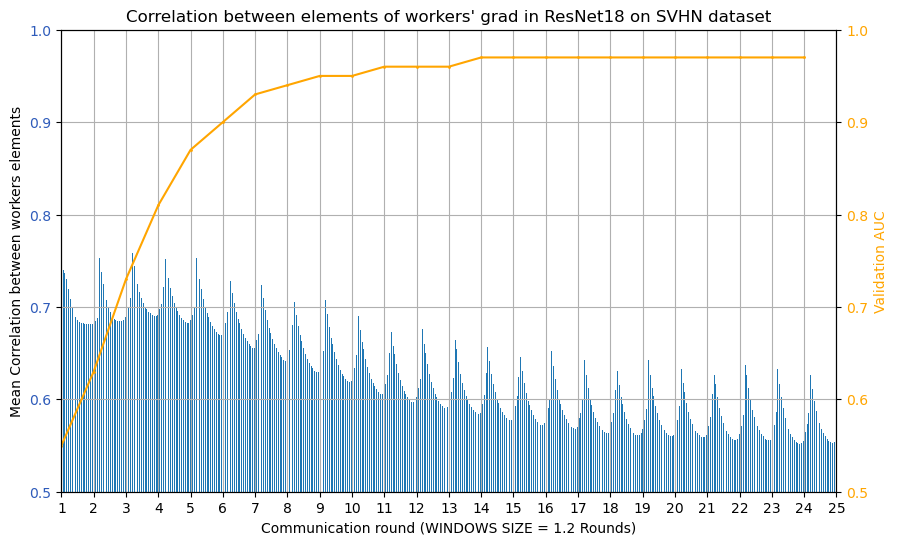
\includegraphics[width=0.7\textwidth]{Chapters/chapter_3_materials_methods/figures/calc correlationpng}
    \caption{Correlation between workers' gradients over time, computed using a sliding window approach to capture meaningful temporal relationships.}
    \label{fig:calc correlation}
\endfigure

\subsection{Distribution Shift}
An important consideration is how the distribution of gradients may shift over time, because the quantizer is sensitive to the shape of the distribution. We'll discuss this more in the 4th chapter.
To assess this, we track the distribution of gradients over time using metrics like KL divergence which can be seen in figure \ref{fig:distribution shift kl div}, as well as visualizing the distributions directly as shown in figure \ref{fig:distribution shift}. as we can see, the general shape of the distribution remains relatively stable, with only minor shifts in the beginning of training.

\figure[htbp]
    \centering
    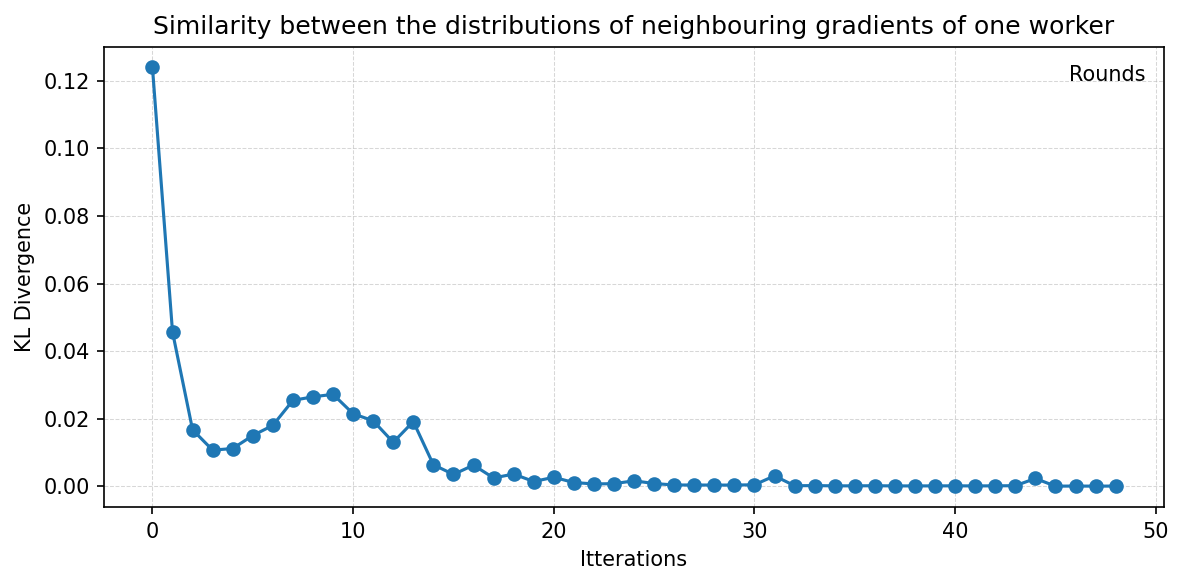
\includegraphics[width=0.7\textwidth]{Chapters/chapter_3_materials_methods/figures/distribution change - kl div}
    \caption{Three different distributions of gradients observed over time, showing very small shifts.}
    \label{fig:distribution shift kl div}
\endfigure

\figure[htbp]
    \centering
    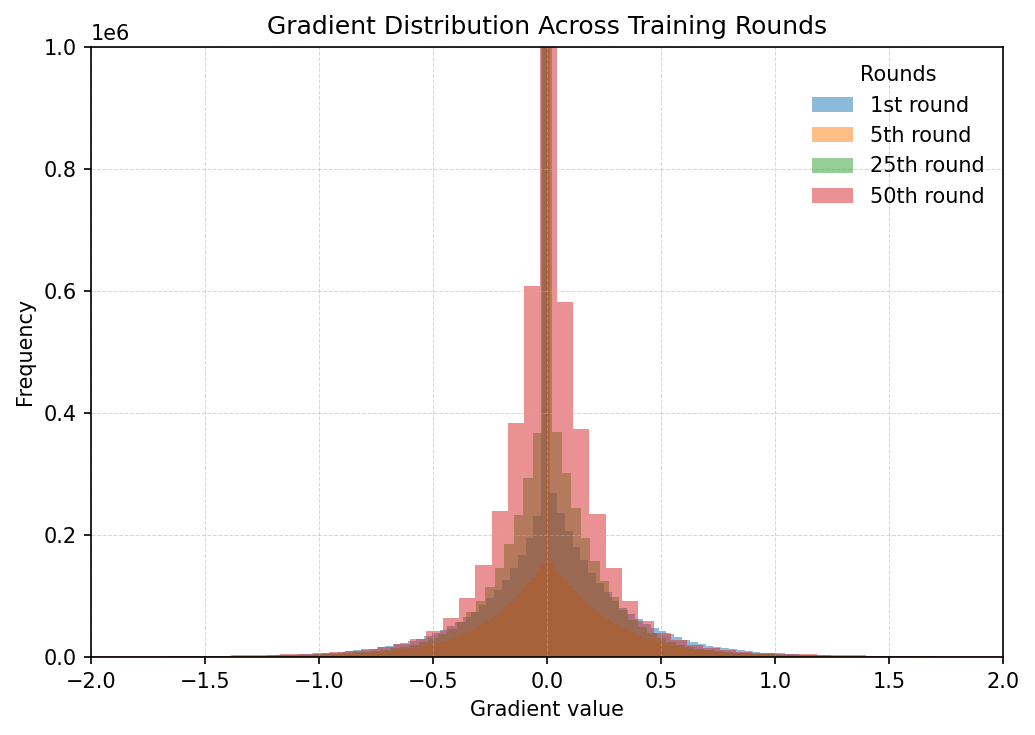
\includegraphics[width=0.7\textwidth]{Chapters/chapter_3_materials_methods/figures/distribution change}
    \caption{Three different distributions of gradients observed over time, showing very small shifts.}
    \label{fig:distribution shift}
\endfigure
